\chapter{Statistical image models}


Building priors for images is an active area of research in which there has been remarkable progress. Understanding the world of images and finding rules that describe what is likely and what is not to find within an image seems like a very challenging task. What we will see in this chapter is that some of the filters that we have seen in the previous chapters have remarkable properties when applied to images.

First we need to understand what we mean by a {\em natural image}. An image is a very high dimensional array of pixels $\img \left[n,m\right]$ and therefore, the space of all possible images is very large. Even if you consider very small thumbnails of $32\times32$ pixels and 3 color channels, with 8 bits per channel, there are more than $10^{7000}$ possible images. Of course, most of them will just be random noise. 

As natural images are quite complex, research started considering simple visual worlds that retained some of the important properties of natural images while allowing developing analytic tools to characterize them.


\begin{figure}[htpb]
\centerline{
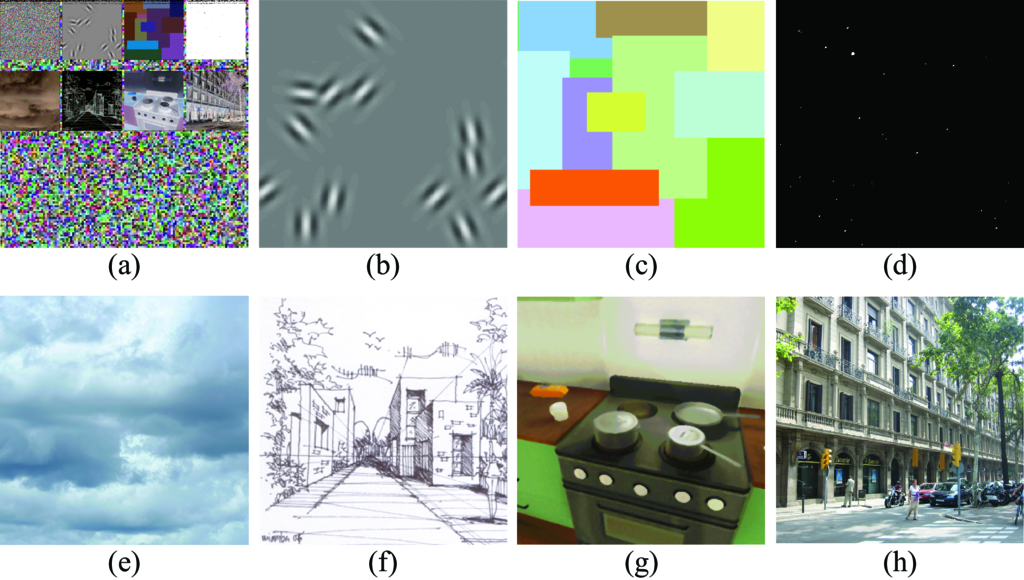
\includegraphics[width=1\linewidth]{figures/statistical_image_models/worlds.eps}
} 
\caption{Different visual worlds, some real, some synthetic. a) white noise, b) stars, c) gabor patches, d) mondrian, e) clouds, f) line drawings, g) CGI, e) a real street. All these worlds have different visual properties. Even there is something that makes CGI images distinct from pictures of true scenes.} 
\label{fig:worlds}
\end{figure}


Figure \ref{fig:worlds} shows images that belong to different visual worlds. 
%
%The first world (fig.~\ref{fig:worlds}.a) is the world of white noise. It is the world that you get to see when you watch an old TV. Images in this world can be easily described by specifying the algorithm used to generate them: create and array of $n \times m$ color pixels and assign to each color component of each pixel a random number drawn from a uniform distribution between 0 and 255. In this world, all the images that belong to this world are very different in terms of the exact RGB values that make every pixel. But all the images look the same to the human visual system. 
%
%The second world (fig.~\ref{fig:worlds}.b) is the world of random Gabor patches. It is a visual world that one gets to see when reading papers on visual psychophysics. Again, an algorithm provides the perfect description for this world: select at random $N$ locations in the image and place at each location,a Gabor patch with a random orientation. These images look a lot more interesting to the human eye even though they contain a lot less detail than images from the first world.  
%
%The third world (fig.~\ref{fig:worlds}.c) is the world of Mondrian paintings. This world is more visually appealing. It contains structures that the eye loves. To the point that some people have made a lot of money by generating samples from this visual world. In its most simplistic form, the images that belong to this set can be described as a random set of squares with random sizes and locations. The squares are drawn in a random order, generating a random pattern of occlusions among them. 
%
%The fourth visual world (fig.~\ref{fig:worlds}.d) is the world of outer space images. This visual world, despite that it appears as being relatively simple, at least visually, it is not. However giving an exact algorithm to produce images from this set is quite challenging, but doable. One good approximation is to generate images by randomly placing a small number of small dots on a black background. A better algorithm will requite modeling star dynamics, gravity, etc.   
%
%The fifth visual world (fig.~\ref{fig:worlds}.e) is the world of clouds. This visual world is visually simple, but it is hard to put into words a description of how images of this set should be generated.  One can describe the images as "pictures of clouds" but that description will be hardly useful. 
%
%The sixth world (fig.~\ref{fig:worlds}.f) is the world of line drawings of real scenes. The images in this set contain a sparse set of thin dark lines on a white background. Going beyond that description is hard. One could also add that the lines are organized to depict real world places and that they seem to correspond to important boundaries of objects in the world. But that definition is not a good procedural description, and it also feels incomplete (some of the lines do not necessarily correspond to object boundaries).  
%
%The seventh world (fig.~\ref{fig:worlds}.g) is the world of realistic scenes rendered with cheap computer graphics. Because the images are generated with computer graphics, there is a procedure that one can follow to generate them. But the procedure lacks the simplicity of the previous visual worlds. The images in this set contain the complexity of real pictures. But there is something missing, something that makes that image to look like what it really is: a cheap CGI. 
%
%The eight world (fig.~\ref{fig:worlds}.h) is the set of typical images that one can take by taking pictures of the real world.  Explaining what makes images in this set different to all other images is not an easy task. 
%
%One important observation is that we can clearly differentiate images as belonging to any of these 8 worlds, even if those visual worlds look like nothing we normally when walking around... 
%
In this chapter we will talk, in some way or another, about all these visual worlds. The goal of this lecture is to present a set of models that can be used to describe images with different properties. We will describe models that can be used to capture what makes special each visual world. Even if the models we will discuss will not be as accurate as the models for the visual worlds a-c, we will show that the models can be descriptive enough to be useful in a number of applications.  These models can be used to separate images into different causes, to do image denoising, superresolution, ...




\begin{figure}[htpb]
\centerline{
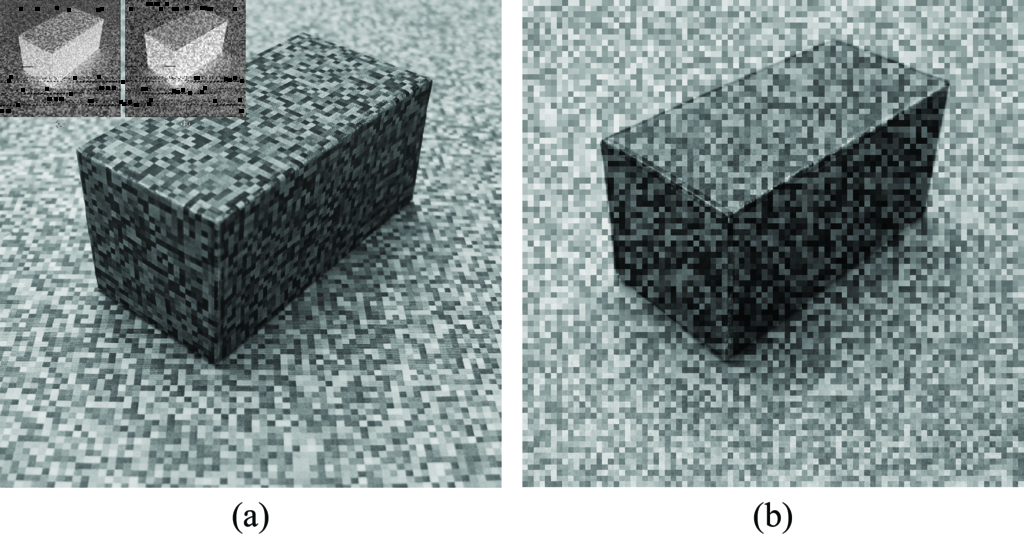
\includegraphics[width=1\linewidth]{figures/statistical_image_models/noiseInTheWorld.eps}
} 
\caption{Telling noise from texture. Which one is which?} 
\label{fig:noiseInTheWorld}
\end{figure}




%\section{Introduction}

% DOCUMENTS:
% lecture 3 (a bit)
% 
%Some history first: models used for TV? JPEG?

%\section{Retinex}
%
%How do you tell gray from white? This might seem like a simple question, but one remarkable aspect of vision is that even the perception of the simplest image and the measurement of the simplest quantity might be far from trivial. 
%
%\begin{figure}[htpb]
%\centerline{
%
\includegraphics[width=1\linewidth]{figures/statistical_image_models/retinex.jpg}
%} 
%\caption{What happens if we see two patches of unknown reflectance, and each illuminated with two different light sources of unknown identity? Simultaneous contrast illusion.} 
%\label{fig:simultaneous}
%\end{figure}
%
%To understand that answering that question is not trivial, let's consider the structure of light that reaches the eye which is the input upon which our visual system will try to differentiate black from white. The amount of light that reaches the eye from painted piece of paper is the result of two quantities: the amount of light reaching the piece of paper, and the reflectance of the surface (what fraction of the light is reflected back into space and what fraction is absorbed by the material).
%
%
%%The brightness of a patch is a function of the light reaching a surface and how much light is reflected by that surface. Under the same illumination, one patch might appear darker than another if it reflects less light. On the other hand, if one patch received more light than other identical patch, the first patch will appear brighter. Therefore, 
%
%
%
%If two patches receive the same amount of light, then we will perceive as being darker the patch that reflects less light. But what happens if we change the amount of light that reaches the scene? What if we increase the amount of light projected on top of the dark patch, what will be see now? What will happen if we have two patches on the same scene each of them receiving different amounts of light? How does the visual system decide what white is and how does it deal with changes in the amount of light illuminating the scene? The visual system is constantly trying to estimate what the incident illumination is and what are the actual reflectances of the surfaces present in the scene. 
%
%If our goal is to estimate the shade of gray of a piece of painted paper, then the quantity that we care about is the reflectance of the surface. But, what happens if we see two patches of unknown reflectance, and each illuminated with two different light sources of unknown identity?  How does the visual system manages to infer what the illumination and reflectances are?
%
%Visual illusions are a way of getting to feel how our own visual system processes images. To experience how this estimation process works let's start considering a very simple image as shown in fig.~\ref{fig:simultaneous}. This image shows a very simple scene formed by a surface with a set of squares of different gray levels illuminated by a light spot oriented towards the left. Our visual system, tries to estimate the two quantities: the reflectance of each square and the illumination intensity reaching each pixel.  
%
%Let's think of the image formation process. The surface is made of patches of different reflectances $R(x,y) \in (0,1)$. Each location receives an illumination $L(x,y)$. The observed brightness is the product:
%\begin{equation}
%\img(x,y) = R(x,y) \times L(x,y) 
%\end{equation}
%
%Despite that what reaches the eye is the signal $\img(x,y)$, our perception is not the value of $\img(x,y)$. In fact, the squares 1 and 2 in fig.~\ref{fig:simultaneous} have the exact same values of intensity but we see them differently which is generally explained by saying that we discount (at least partially) the effects of $L(x,y)$. 
%
%But how can we estimate $R(x,y)$ and $L(x,y)$ by only observing $\img(x,y)$? One of the first solutions to this problem was the Retinex algorithm proposed by Land and McCann. Land and McCann observed that it is possible to extract $R$ and $L$ from $\img$ if one takes into account some constraints about the expected nature of the images $R$ and $L$. Land and McCann noted that if one considers two adjacent pixels inside one of the patches of uniform reflectance, the difference between the two pixel values will be very small as the illumination, even if it is nonuniform, will only produce a small change in the brightness of the two pixels. However, if the two adjacent pixels are in the boundary between two patches of different reflectances, then the intensities of these two pixels will be very different. 
% 
%The Retinex algorithm works by first extracting x and y spatial derivatives of the image $\img(x,y)$ and then thresholding the gradients.  First, we transform the product into a sum using the $\log$:
%
%\begin{equation}
%\log \img(x,y) = \log R(x,y) + \log L(x,y) 
%\end{equation}
%Taking derivatives a long $x$ and $y$ is now simple:
%\begin{equation}
%\frac{\partial \log \img(x,y)}{ \partial_x} = \frac{\partial \log R(x,y)}{ \partial_x} + \frac{\partial \log L(x,y)}{ \partial_x} 
%\end{equation}
%
%Any derivative larger that the threshold is assigned to the reflectance image $R(x,y)$ and the ones smaller than a threshold are assigned to the illumination image $L(x,y)$
%
%\begin{equation}
%\frac{\partial \log R(x,y)}{ \partial_x} =  \left\{
%\begin{array}{rl}
%\frac{\partial \log \img(x,y)}{ \partial_x} & \text{if} ~  \left| \frac{\partial \log \img(x,y)}{ \partial_x} \right|>T\\
%0 ~~~~~~~~& \text{otherwise}
%\end{array} \right.
%\end{equation}
%
%\begin{figure}[htpb]
%\centerline{
%\includegraphics[width=1\linewidth]{figures/statistical_image_models/retinex_solution_b.eps}
%} 
%\caption{Derivatives classified into reflectance or luminance components.} 
%\label{fig:simultaneous2}
%\end{figure}
%
%and doing the same thing from $ \partial_y$. Then, the image $\log R(x,y)$ is obtained by integrating the gradients and exponentiating the result. Finally, the illumination can be obtained as $L(x,y) = \img(x,y)/R(x,y)$.
%
%\begin{figure}[htpb]
%\centerline{
%\includegraphics[width=1\linewidth]{figures/statistical_image_models/retinex_solution_a.eps}
%} 
%\caption{Recovered components.} 
%\label{fig:simultaneous3}
%\end{figure}
%
%Note that the illumination derivatives have much lower magnitude than the reflectance derivatives, however they extend over much larger spatial regions which makes that once they are integrates, changes in brightness due to no-uniform illumination might be larger than changes due to variations in reflectance values. 
%
%Despite the simplicity of this approach it works remarkable well with images like the ones shown in fig.~\ref{fig:simultaneous} and also with a number of real images. However, the algorithm is limited and it is easy to make it fail in situations were the visual system works as we will see later in more depth.
%
%The Retinex algorithm works by making assumptions about the structure of the images it tries to separate. The underlying assumption is that the illumination image $L(x,y)$ varies smoothly and the reflectance image $R(x,y)$ is composed of uniform regions separated by sharp boundaries. These assumptions are very restrictive and will limit the domain of applicability of such an approach. Understanding the structure of images in order to build models such as Retinex has been the focus of a large amount of research. This chapter will introduce some of the most important image models.
%
%The recovered brightness is stronger than what we perceive. There are a number of reasons that weaken the perceived brightness. The effect is bigger if the display occupies the entire visual field. Right now the picture appears in the context of the page which also affects the estimation of the illumination. Also, the two larger squares do not seem to group well with the rest of the display, as if they were floating in a different plane. And finally, for such a simple display, the visual system does not fully separate the perception of both components. 
%

%CNNs try to learn what to do with images to solve a task.

%In this chapter, we describe techniques in which researchers try to derive how to do process images using simple principles about the real world. Under some assumptions the solutions are optimal (although the assumptions are often wrong).




%Example 1: Retinex: Mondrian world with a illumination ramp. 


%FROM TED: Land and McCann began by considering the nature of
%scenes and images. They argued that reflectance tends to be
%constant across space except for abrupt changes at the transitions
%between objects or pigments. Thus a reflectance
%change shows itself as step edge in an image, while illuminance
%will change only gradually over space. By this argument
%one can separate reflectance change from illuminance
%change by taking spatial derivatives: high derivatives are due
%to reflectance and low ones are due to illuminance.
%The Retinex model applies a derivative operator to the
%image, and thresholds the output to remove illuminance variation.
%The algorithm then reintegrates edge information over
%space to reconstruct the reflectance image.
%
%Helmholtz, who argued that perception is the product of
%unconscious inference. His dictum was this: what we perceive
%is our visual systemÕs best guess as to what is in the
%world. The guess is based on the raw image data plus our
%prior experience. In the Helmholtz view, lightness constancy
%is achieved by inferring, and discounting, the illuminant.
%
%We use the term atmosphere to
%refer to the combined effects of a multiplicative process
%(e.g., illuminance) and an additive process (e.g., haze). It turns out that most physical effects will
%lead to linear transforms. Therefore the combined effects can
%be captured by a single linear transform (characterized by
%two parameters). This is what we call an atmosphere.

% Retinex works by thresholding the gradients and assigning
%the gradients below the threshold to the gradients of the
%illumination image.



%Example 2:

%This problem has an even simpler version. 

% Gray scale constancy



% There is an analogy to make with language models. They also look for generative models of language. The statistical models are very similar. 

%TO ADD:
%
%- Intrinsic images
%
%- Frameworks of illumination
%
%- Anchor theory
%
%- Failures of the simple mechanism: Kersten images
%
%- What seems white now, might appear gray if something whiter appears on the same scene. 


%\section{Separating images into components}
%
%%\begin{figure}[htpb]
%%\centerline{
%%\includegraphics[width=1\linewidth]{figures/statistical_image_models/mixtures3_a.eps}
%%} 
%%\caption{The goal is to separate each image into several images.} 
%%\label{fig:mixtures}
%%\end{figure}
%
%One of the reasons why it is interesting to understand the properties of different sets of images is because many perceptual tasks can be formulated as separating an input image into a collection of images, each one describing a different image property. %Figure \ref{fig:mixtures} shows three additional examples of images that have are made of multiple components.  
%
%%The first example shows a normal photograph corrupted by noise. 
%
%\begin{figure}[htpb]
%\centerline{
%\includegraphics[width=1\linewidth]{figures/statistical_image_models/mixtures3_noise.eps}
%} 
%\caption{The goal is to separate each image into several images.} 
%\label{fig:mixtures}
%\end{figure}
%
%\begin{equation}
%\img_n(x,y) = \img(x,y) + n(x,y)
%\end{equation}
%
%Our visual system is able to notice that this image is not normal and that it is corrupted by noise. We do not perceive this scene as being composed by objects covered with a strange form of paint. We see that there is {\em noise} and it is not supposed to be there, it is not part of the real scene. What we will like is to be able to remove the noise from the image automatically. This is equivalent to be able to separate the image into two components, one looking like a clean uncorrupted picture of a street and the second image containing only noise. 
%
%How do we tell noise from texture? Figure~\ref{fig:noiseInTheWorld} shows two scenes one contains noise, and the other objects textured with noise. Can you tell which one is which? Where is the noise? in the image or in the world?  Image noise does not follow the objects, does not deform with the 3D surfaces, it does not change frequency with distance, ... If the noise was really in the world, stationary noise will require a special noise distribution that conspires with the observer view point to appear stationary.
%
%The second example shows a blurry image. 
%
%\begin{figure}[htpb]
%\centerline{
%\includegraphics[width=1\linewidth]{figures/statistical_image_models/mixtures3_blur.eps}
%} 
%\caption{The goal is to separate each image into several images.} 
%\label{fig:mixtures}
%\end{figure}
%
%\begin{equation}
%\img_b(x,y) = \img(x,y) \circ g(x,y) 
%\end{equation}
%
%This image can be decomposed into a full resolution image from which we remove the high spatial frequencies from it. Again, we do not perceive the blurry image as a normal picture of a scene composed by objects with fuzzy boundaries. 
%
%
%and the third image is the sum of two normal images (additive transparency). Again, we have a very vivid impression of transparency. 
%
%\begin{figure}[htpb]
%\centerline{
%\includegraphics[width=1\linewidth]{figures/statistical_image_models/mixtures3_transparency.eps}
%} 
%\caption{The goal is to separate each image into several images.} 
%\label{fig:mixtures}
%\end{figure}
%
%\begin{equation}
%\img_t(x,y) = \img_1(x,y) + \img_2(x,y) 
%\end{equation}
%
%Separating an image into different causes it is an important vision task.  It is important to note that the separation into these components does not rely on our ability to recognize objects and scenes (at least not totally). It seems to rely on more basic mechanisms. These tasks can not be solved without making some assumptions about the nature of the composing images. 

%The problem we are trying to solve is like trying to find $a$ and $b$ given the next equation:
%\begin{equation}
%1 = a \times b
%\end{equation}
%
%Compare this with the prototypical graphics problem: here are two numbers $a$ and $b$;  what is their product?
%
%In the rest of the chapter we will see models of images that will provide useful tools to separate images into components. 
%
%
%
%
%\section{Bayesian inference}
%
%In many situations in vision we observe some complicated function of the world 
%\begin{equation}
%observation = f(world)
%\end{equation} 
%It would be nice if one could simply do $world = f^{-1}(observation)$, and, in some cases, this is possible. But in general, inverting this function might be very difficult, or ill-posed. As we saw before, in many important cases, there are multiple $worlds$ that give raise to the same $observations$. We need to find a way of inverting this function. Bayesian inference provides the set of tools to regularize the solution and to add priors. It also provides the tools to deal with uncertainty due to noise in our observations. Let's see how we can use Bayesian inference to find the solution to the typical vision problem $ab=1$.
%
%%Introduce Bayes
%
%%Introduce notation with random variables
%
%%Talk about inference and Helmholtz
%
%%A way of dealing with uncertanty
%
%%A way of doing function inversion when the problem is under constrained. One example: the typical vision problem $ab=1$:
%
%%\example{Grayscale constancy}
%%
%%
%%Conclude making a simple image example to help introducing the interest of a model of an image prior. In the case of images, we can have:
%%
%%\begin{equation}
%%p(\img) = 
%%\end{equation}
%%
%%
%%The problem $ab=1$ is quite typical in vision. Let's consider a real vision problem. 
%%
%%Let's consider the image from figure XXX. This image is composed by a set of squares with different levels of gray. One of them is perceived as white. However, how is that we see that square as being white? Despite that this might seem trivial, it is not once we consider how the image that reaches our eye is formed.
%%
%%What we see is the product of
%%
%%\begin{equation}
%%[k_1, k_2, ..., k_n] = a [b_1,b_2, ..., b_N]
%%\end{equation}
%% To find $L$ and the sequence of reflectances $b_1, ..., b_N$ we are going to need to make some assumptions.
%% 
%%Suppose all reflectances $b_i$ are uniformly distributed between 0 and 1.  
%%
%%\begin{equation}
%%p(b_1, b_2, ..., b_N) =   \left\{
%%\begin{array}{rl}
%%1 & \text{if } 0<b_i <1\\
%%~ & ~\\
%%0 & \text{otherwise}
%%\end{array} \right.
%%\end{equation}
%%
%%
%%Suppose you observe N image intensities, which is the product of those N reflectance draws
%%times some unknown illumination $L$ (with $L>0$).  If we can estimate the reflectance
%%of the brightest patch, then we can calculate the unknown illumination
%%value, and then the reflectance of every patch.  
%%
%%
%%For N reflectance draws, we can calculate the probability that the
%%brightest of those N draws has a reflectance of x.  That's the same as
%%the probability that every reflectance draw is x or lower, which is
%%$x^N$.  As the number of observed reflectances, N, gets bigger and
%%bigger, it becomes a better and better bet that the brightest of those
%%patches is white. This is true even for an arbitrary distribution of reflectances between 0 and 1. 
%%
%%why not to look for the average gray? That could be more reliable than everything as it would not depend on any maximum value. I think that the problem of using the average is that then it will not be distribution independent. Using the max value is distribution independent.
%%
%%It's interesting to think through what breaks the symmetry (black/white):  why not look for the blackest patch and call it "black".     (a) there is no value of "black", as there is a value for white, 1.0.  Should it be a reflectance of 0.001?  0.00001?   and (b) so then knowing which intensity is black doesn't tell you what the light intensity is, because you can't divide the observed intensity by the unknown value of black to find the illumination intensity.
%%
%%
%%
%%Using the average gray is certainly a standard algorithm.  I believe the reference for that is Buchbaum,
%%G. Buchsbaum. A spatial processor model for object colour
%%perception. J. Franklin Inst., 310:1{26}, 1980.
%%
%%And I guess a reference for bright=white could be some Retinex paper.  They don't justify it, but they certainly use that assumption.
%%So maybe this:  E. H. Land. The retinex theory of color vision. Sci. Am.,
%%237(6):108{128}, 1977
%%
%%
%%And indeed, our visual system seems to follow that reasoning.  If you see a greater variation of patch values, intensity illusions that rely on the bright=white assumption get stronger and stronger (some of Ted's brightness illusions).
%%
%%FIGURE: Frameworks of illumination: figure with two sets of randomly colored patches, with a division between them. In the left [0,0.5] and in the right [0,1]. We will see a vertical shadow. And we will see the right white from each side. 
%%
%%
%%
%%\begin{figure}[htpb]
%%\centerline{
%%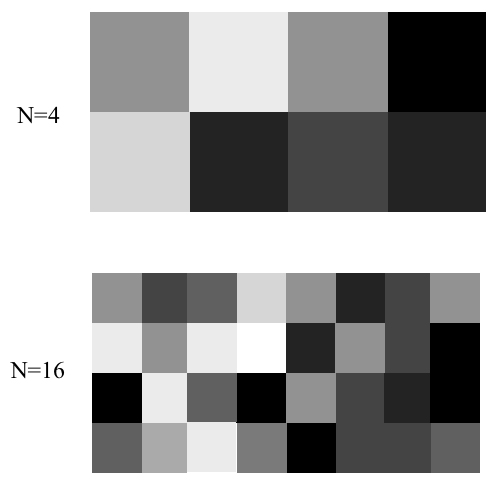
\includegraphics[width=.6\linewidth]{figures/statistical_image_models/chips.jpg}
%%} 
%%\caption{Here is an example showing the effect of the number of independent samples, N, on the estimate of illuminations and reflectances.  For N=4, there aren't quite enough samples to decide on regions of uniform illumination, while for N=16, you start to get the sense that the right hand side is in shade.  Maybe including N=64 would make it completely clear.} 
%%\label{fig:chips}
%%\end{figure}
%%
%%
%
%%\section{Gestalt}
%%
%%%The
%%%key concepts include grouping, belongingness, good continuation,
%%%proximity, and so on.
%%
%%Can we introduce grouping theories as particular instances of statistical image models?
%%
%%
%%The problem is that to use these statistics we need to detect some tokens on the image (edges, junctions, ...). We will see how to do this later, but even with the most accurate detectors, the output is still unreliable. In the rest of the chapter we will study a different class of statistical image models that do not require taking premature decisions about the image content. 
%
%%\section{Accidental alignments}
%%
%%
%%where do we talk about accidental alignments? Isn't this also part of statistical image models?
%%
%%This is a good example on the power of statistical models to solve hard tasks. 
%%
%
%




\section{A sequence of statistical models of images}

There is a significant interest in building image models that can represent whatever makes special real photographs relative to, let's say, images that just contain noise. One way of building an image model is by having some procedural description, for instance a list of objects with locations, poses and styles and a rendering engine, just like one would do when writing a program to generate CGI. One issue with this way of modeling images is that it will be hard to use it, and will require having an exhaustive list of all the things that we can find in the world. We will see later in the class that the apparent explosion in complexity should not stop us. 


% Drawing the blocks of first level:
\centerline{
\tikzset{
  block/.style    = {draw, thin, rectangle, minimum height = 2.5em,  minimum width = 2.5em},
  sum/.style      = {draw, circle, minimum size=.4cm}, % Adder
  input/.style    = {coordinate}, % Input
  output/.style   = {coordinate}, % Output
  x/.style   = {coordinate} % Output
}
\begin{tikzpicture}[auto, thin, node distance=1.2cm, >=triangle 45]
\draw
	node [] (x0p) {$x$}
	node [block, right of=x0p] (f) {$f$}
	node [right of=f, node distance=2.6cm] (out) {$p(x \in World)$};
       % Joining blocks. 
	\draw[->](x0p) -- node {} (f);
	\draw[->](f) -- node {} (out);
\end{tikzpicture}
}
However there is another way of building image models. In the rest of this lecture we will study a very different approach that consists in building statistical models of images that try to capture the properties of small image neighborhoods. Statistical models are very successful in other disciplines such as natural language modeling.

Here we will review models of images of increasing complexity starting with the simplest possible neighborhood: {\em the pixel}.


\subsection{Histograms}

The simplest image model will consist in assuming that all pixels are independent and their intensity value is drawn from some distribution. We can write this as:
\begin{equation}
p(\img) = \prod_{x,y} p(\img(x,y))
\label{eq:histmodel}
\end{equation}
We will see the interest of writing models in this form. One way of getting a sense of how accurate is a statistical image model is to sample from this model and check the types of images that it produces. This will require knowing the distribution $p(\img(x,y))$ (we will assume this function is the same in all image locations). What we can do is to take one image from one of the visual worlds that we described in the introduction, we can then estimate the function $p(\img(x,y))$ as the histogram of the image. We can then sample new images from eq.~\ref{eq:histmodel}.  Figure~\ref{fig:histMatch} shows two pairs of images with matched intensity histograms. We can see that this simplistic model is somewhat appropriate for pictures of stars (although star images can have a lot more structure), but it miserably fails in reproducing anything with any similarity to a street picture. 


\begin{figure}[htpb]
\centerline{
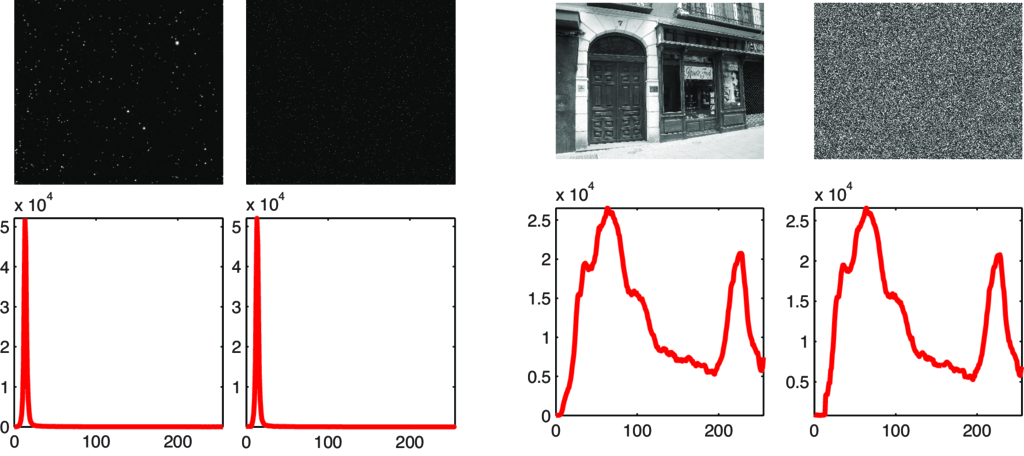
\includegraphics[width=1\linewidth]{figures/statistical_image_models/spaceHist.eps}
} 
\caption{Examples of images and white noise with matched histograms. Only the image with stars has some visual similarity with pictures of stars.} 
\label{fig:histMatch}
\end{figure}

Let's be honest, as a generative model of images, this model is very poor. However, this does not mean that image histograms are not important. Manipulating image histograms is a very useful operation.  Given two images $\img_1$ and $\img_2$ with histograms $h_1$ and $h_2$, we look for a pixelwise transformation $f(x)$ so that the histogram of the transformed image, $f(\img_1)$, matches the histogram of $\img_2$. There are many ways in which histograms can be transformed. One natural choice is a transformation that preserves the ordering of pixels intensities. 
%
%Figure~\ref{fig:illumination} shows examples of spheres that are reflecting some complex ambient illumination. The two spheres on the left are the two original images. The ones on the left are generated by modifying the image histograms to match the histogram of the opposite image.  The figure shows that by simply changing the image histogram we can transform how we perceive the material of each sphere: from shiny to mate.
%
%
%\begin{figure}[htpb]
%\centerline{
%\includegraphics[width=1\linewidth]{figures/statistical_image_models/illuminationHistograms.eps}
%} 
%\caption{This is an example that illustrates the perceptual importance of simple histogram manipulations. Note how by simply modifying the image histograms, the sphere seems to be made by a different type of material. Image from Dror, Fleming, Adelson.} 
%\label{fig:illumination}
%\end{figure}
%
%
%
%

\subsection{Dead leaves model}

\begin{figure}[htpb]
\centerline{
\includegraphics[width=1\linewidth]{figures/statistical_image_models/correlation.eps}
} 
\caption{Scatter plots of pairs of pixels intensities as a function of distance, and cross-correlation function for vertical and horizontal displacements.} 
\label{fig:correlation}
\end{figure}

In the quest to find what makes photographs of everyday scenes special, the next simplest image structure is a set of two pixels. Things get a lot more interesting now. One interesting observation is that if one plots the value of the intensity of one pixel as a function of the intensity value of the pixel nearby, The scatterplot produced by many pixel pairs (fig.~\ref{fig:correlation}) is concentrated on the identity line. As we look at the correlation between pixels that are farther away, the correlation value slowly decays. The correlation between two pixels is:
\begin{equation}
C(\Delta x, \Delta y) = \rho \left[ \img(x+\Delta x,y+ \Delta y), \img(x, y) \right]
\end{equation}

The behavior of this correlation function when computed on natural images is very different from the one we would observe if the correlation was computed over noise images. 

There has been a large number of efforts trying to model what is the minimal set of assumptions that one needs to make in order to reproduce the observed behavior. The {\em dead leaves model } is a simplified image formation model that tries to approximate some of the properties observed for natural images. This model was introduced in the 60's by Matheron (67) and popularized by Ruderman (97). This model consist in assuming that an image can be modeled as a set of disks (dead leaves) that fall on a flat surface generating a random superposition (e.g., fig.~\ref{fig:worlds}.c). 

\begin{figure}[htpb]
\centerline{
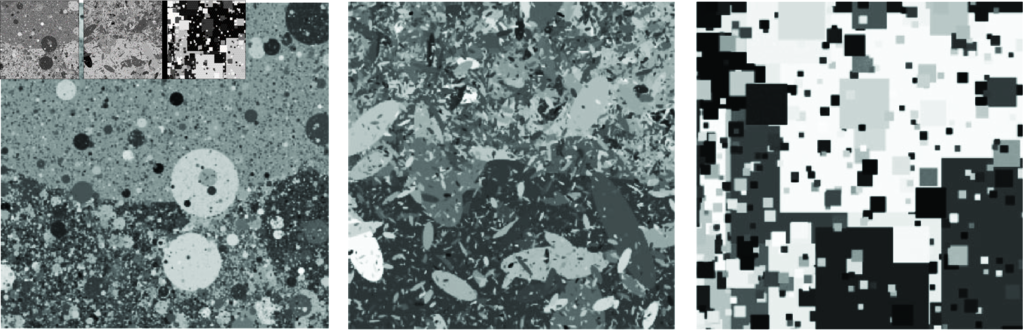
\includegraphics[width=1\linewidth]{figures/statistical_image_models/deadleaves.eps}
} 
\caption{Images resulting from the dead leaves model.
%BUILD SOME CUSTOM MADE IMAGES THAT CORRESPOND TO SOME INTERESTING VARIANTS.  For example: additive, occlusions, scale invariant and plot the measured correlation functions.
} 
\label{fig:deadleaves}
\end{figure}

This model is very simple and does not produce realistic images, but it is similar to the image model assumed to explain the distribution of albedos in natural images. This model is used by the Retinex algorithm to separate and image into two components: illumination and albedo variations. %We will see this later.

The particular form of the correlation function for natural images is made more explicit when studied on the Fourier domain. One remarkable property of most natural images is that if you take the 2D Fourier transform of an image, and look at the form of the magnitude seems to follow a form:
\begin{equation}
| \imgfft(v) | \simeq \frac{1}{| v | ^ \alpha}
\end{equation}
where $v$ denotes spatial frequency, $\imgfft$ is the Fourier transform of the image $\img$, and $\alpha \simeq 1$. And this is true for all orientations (you can think of this as taking the fourier transform and looking at the profile of a slice that passes by the origin). 

%FIGURE: the average fourier transform of natural images and sections.

%FIGURE: noise FT and see you can see differences in the type of textures. 

\subsection{The gaussian model}

We want to write a statistical image model that takes into account the correlation statistics of natural images (see Simoncelli 2005 for a review). If the only constraint we have is the correlation function among image pixels, then, among all the possible distributions the one that has the maximum entropy (maximum entropy principle) is the Gaussian distribution: 
\begin{equation}
p(\img) \propto \exp \left(-\frac{1}{2} \img^T {\bf C}^{-1} \img \right)
\label{eq:gaussianmodel}
\end{equation}
where ${\bf C}$ is the covariance matrix of all the image pixels. Note that now this model does not assume independency across pixels any more. This model takes into account that intensity values for different pixels are correlated as discussed in the previous sections. This model is related also to studies that use principal component analysis to study what are the typical components of natural images. For stationary signals, the matrix ${\bf C}$ has a circulant structure (assuming a tiling of the image) and can be diagonalized using the Fourier transform. The eigenvalues of the diagonal matrix correspond to the power (squared magnitude) of the frequency components of the Fourier transform. This is, the matrix ${\bf C}$ can be written as ${\bf C} = ${\bf E}{\bf D}${\bf E}^T$, where ${\bf E}$ is the matrix that contains the Fourier basis (as seen in the previous lecture) and the diagonal matrix ${\bf D}$ is composed by the values $\frac{1}{| v | ^ \alpha}$ for all the frequencies $v$.
% http://ee.stanford.edu/~gray/toeplitz.eps


%The gaussian model is the result of making a number of assumptions about images:
%
%\begin{itemize}
%\item Stationarity
%\item Scale invariance
%\end{itemize}


\subsubsection{Sampling images}

Once a distribution is defined, we can use it to sample new images. First we need to specify the parameters of the distribution. In this case, we need to specify the matrix ${\bf C}$. We can estimate this as the average covariance matrix of a set of images. Figure \ref{fig:synthClouds} shows an example of an image of clouds and the magnitude of its Fourier transform. A sample of the distribution can be obtained by filtering white gaussian noise using the image magnitude as a filter. 

\begin{figure}[htpb]
\centerline{
\includegraphics[width=1\linewidth]{figures/statistical_image_models/synthClouds.eps}
} 
\caption{Randomizing the phase of picture of clouds. Left) clouds, Center) magnitude of its Fourier transform, Right) image obtained by randomizing the phase.} 
\label{fig:synthClouds}
\end{figure}



\begin{figure}[htpb]
\centerline{
\includegraphics[width=1\linewidth]{figures/statistical_image_models/examplefailurehair.eps}
} 
\caption{BUILD database of hair images and estimate average spectrum.} 
\label{fig:hair}
\end{figure}


%
%\begin{figure}[htpb]
%\centerline{
%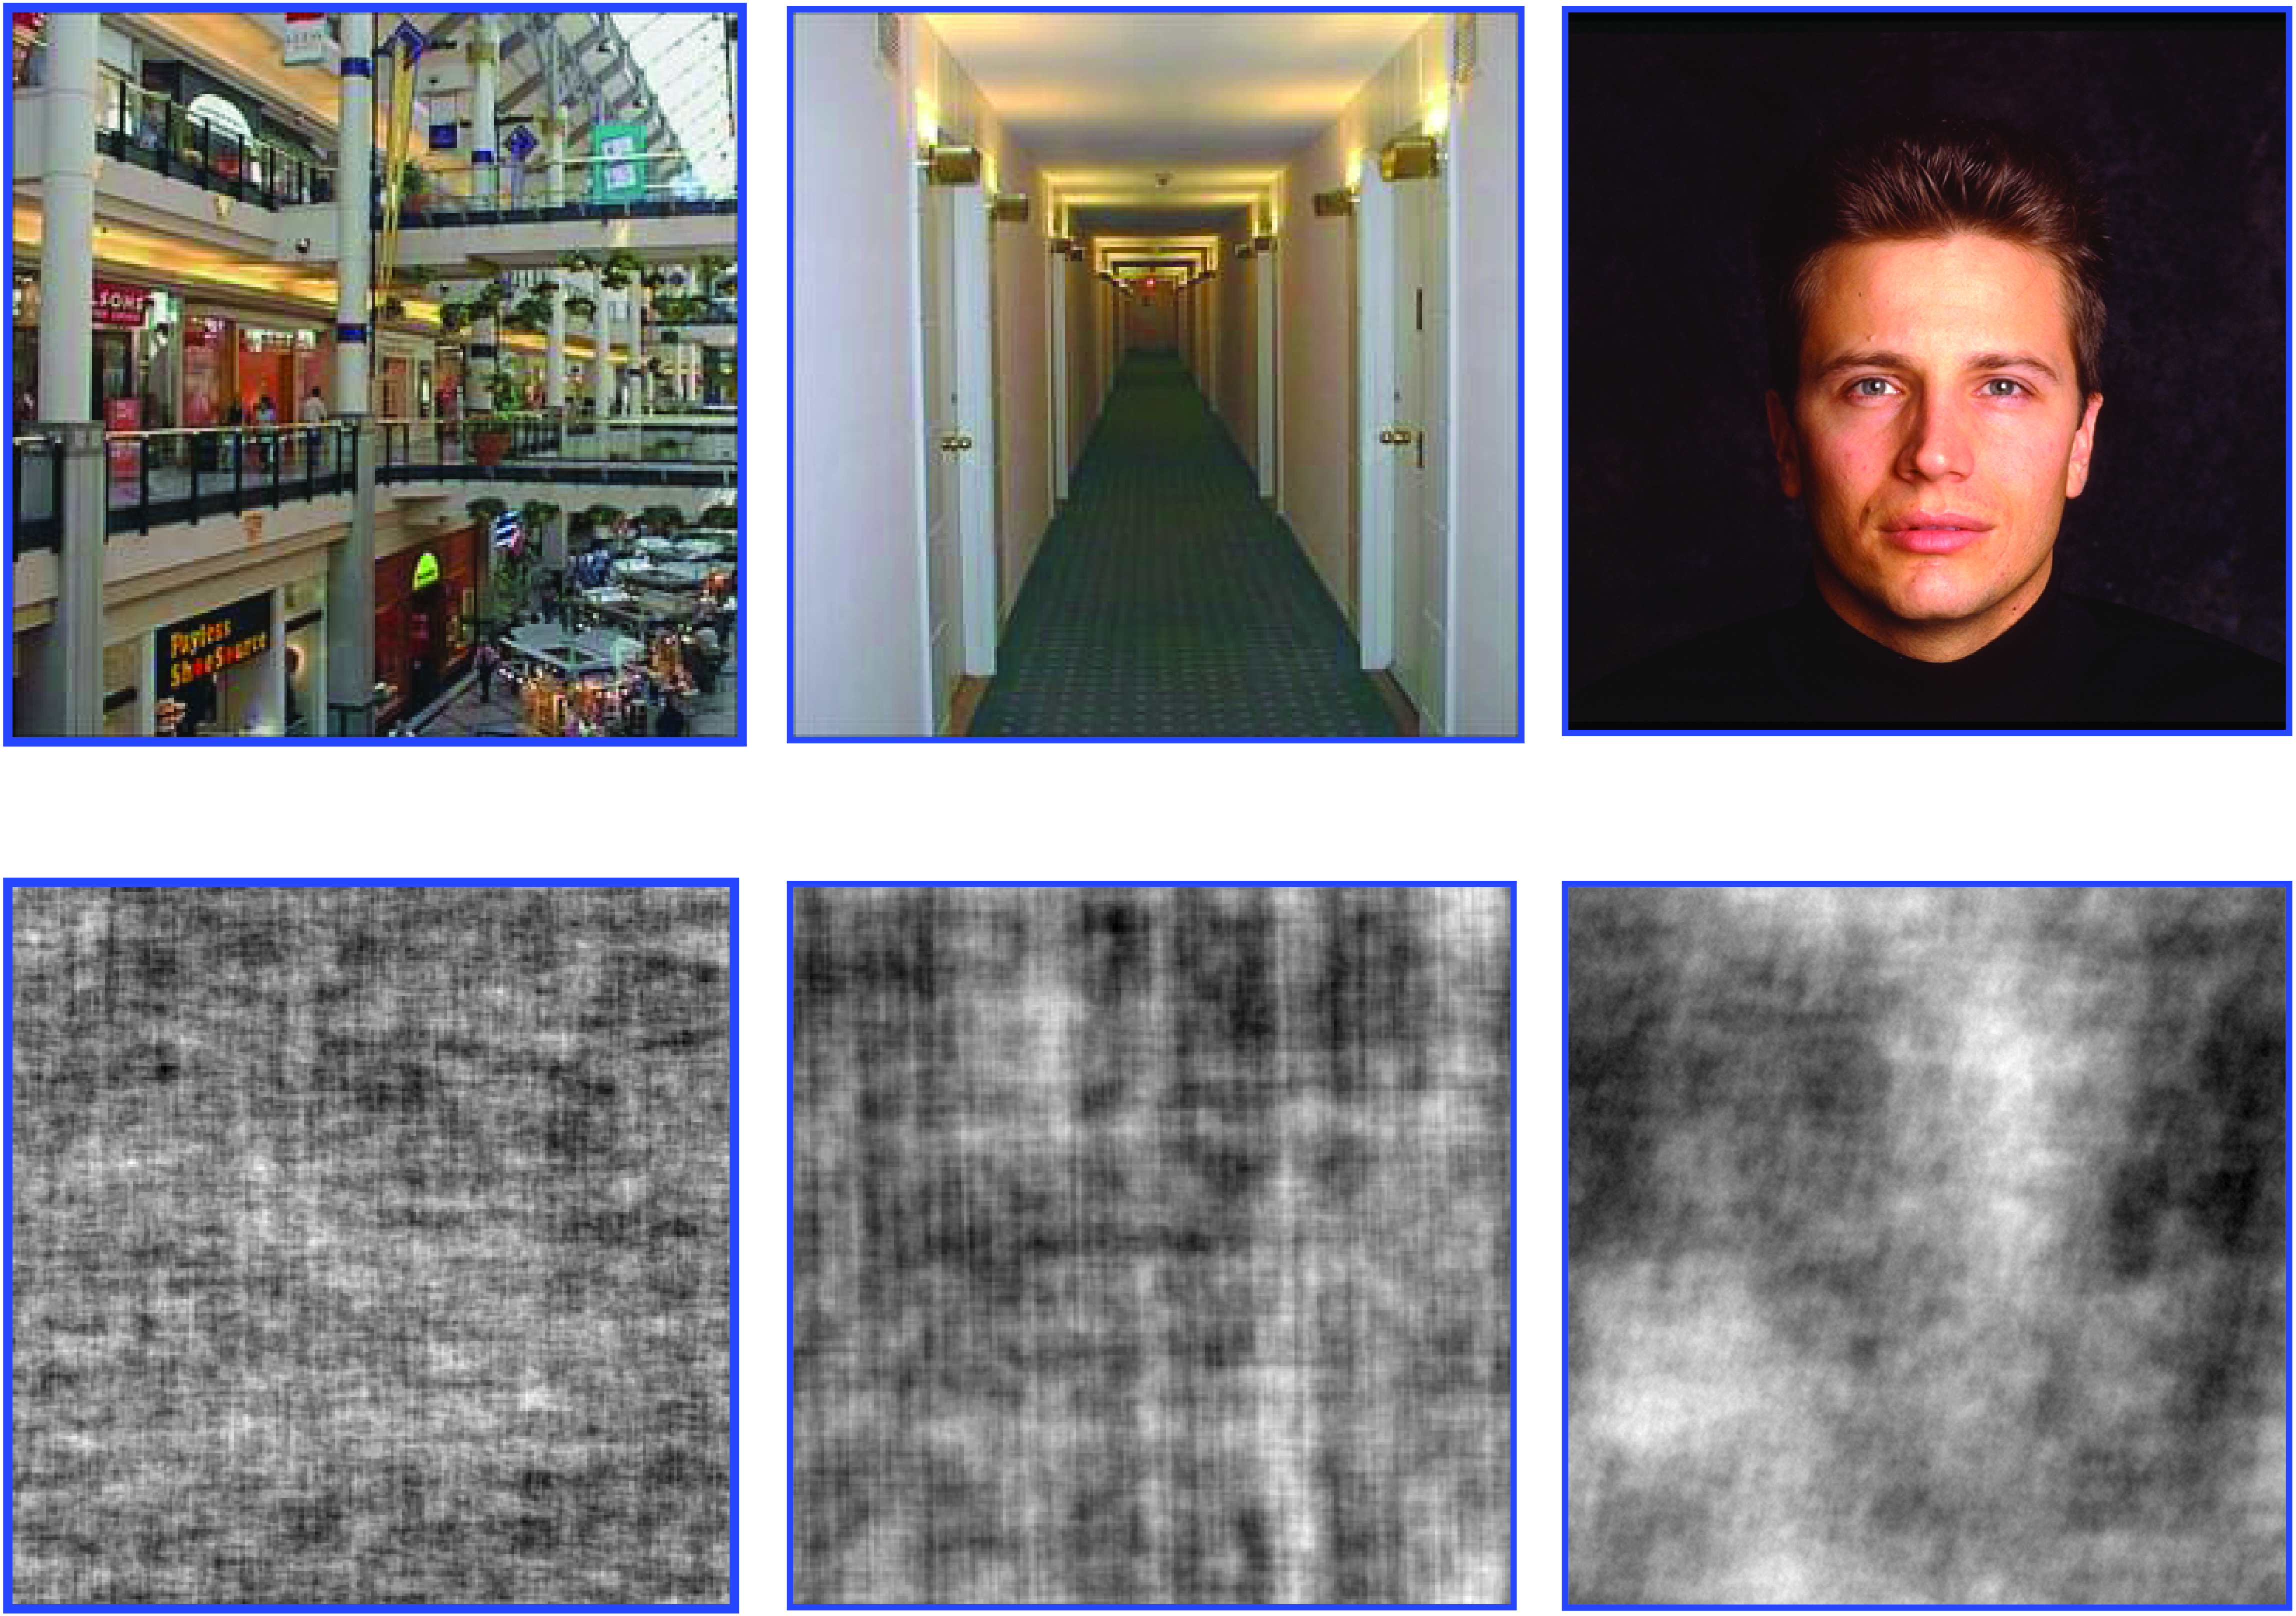
\includegraphics[width=1\linewidth]{figures/statistical_image_models/phaserandomization.eps}
%} 
%\caption{BUILD MORE DISTINCT IMAGES: face, beach, forests with vertical trees.} 
%\label{fig:phaserandomization}
%\end{figure}
%
%

\subsubsection{Image denoising and Wiener filter}
~\\

As an example of how to use image priors for vision tasks, we will study how to do image denoising using the prior on the structure of the correlation of natural images. In this problem, we observe a noisy image $\img_n$ corrupted with white gaussian noise: 
\begin{equation}
\img_n(x,y) = \img(x,y) + n(x,y)
\end{equation}
and the goal is to recover the uncorrupted image $\img(x,y)$. The noise $n(x,y)$ is white gaussian noise with variance $\sigma_n^2$.

The denoising problem can be formulated as finding $\img$ that maximizes the maximum a posteriory (MAP estimate):
\begin{equation}
\max_\img p(\img | \img_n) 
\end{equation}

In these equations we write the image as a column vector $\img$. This posterior density can be written as:
\begin{equation}
\max_\img p(\img | \img_n) = \max_\img p(\img_n | \img) p(\img)
\end{equation}
where the likelihood function is:
\begin{equation}
p(\img_n | \img) \propto \exp( - \left| \img_n - \img \right| ^2 / \sigma_n^2)
\end{equation}
and the prior:
\begin{equation}
p(\img) \propto \exp \left(-\frac{1}{2} \img^T {\bf C}^{-1} \img \right)
\end{equation}

The solution to this problem can be obtained in closed form:
\begin{equation}
\img = {\bf C} \left( {\bf C} + \sigma_n^2   \mathbb{I} \right)^{-1} \img_n
\end{equation}
This is just a linear operation. It can also be written in the Fourier domain as:
\begin{equation}
\imgfft(v) = \frac{A/|v|^{2\alpha}}{A/|v|^{2\alpha} + \sigma_n^2} \imgfft_n(v) 
\end{equation}


\begin{figure}[htpb]
\centerline{
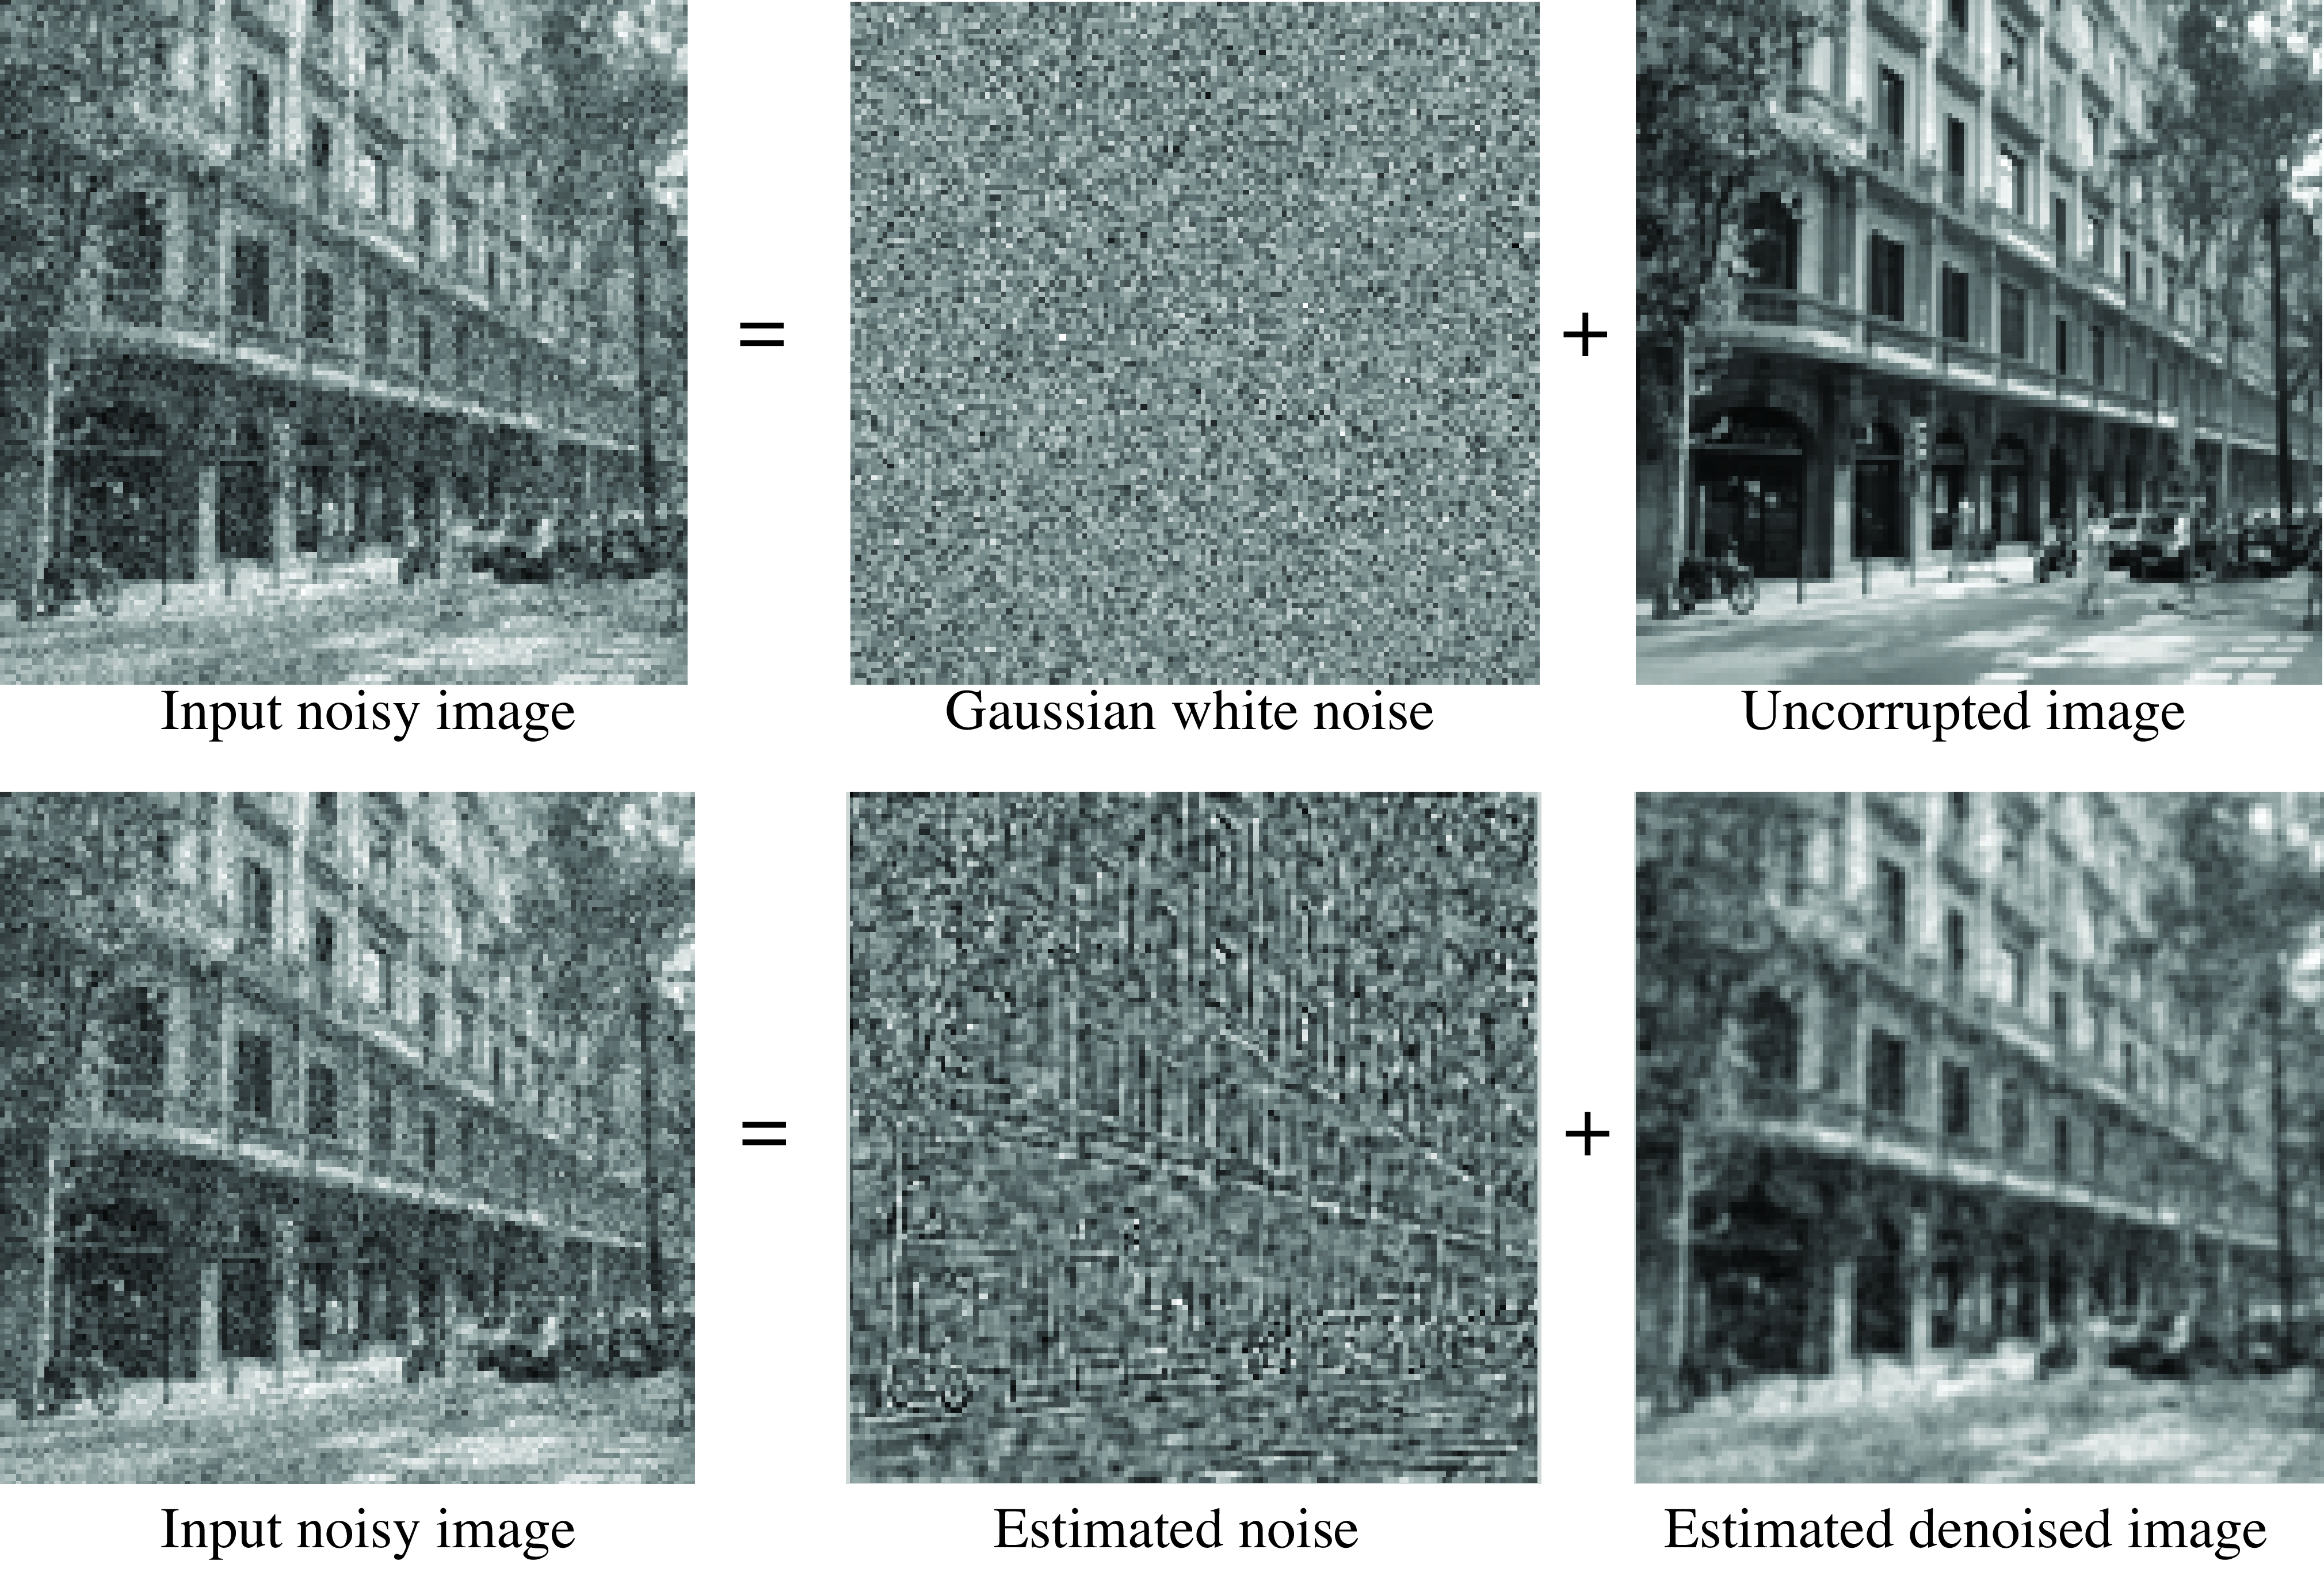
\includegraphics[width=1\linewidth]{figures/statistical_image_models/denoisingGaussianModel.eps}
} 
\caption{In the estimated noise we can see still structure from the original image.} 
\label{fig:denoisingGaussianModel}
\end{figure}






%As a representation, the fourier transform makes explicit the dominant image orientations, the image scales, periodic patterns, ...


%FIGURE: stats for man-made vs. natural. Average spectrum. Explain phase is great to reconstruct image, but the magnitude, as a representation makes information explicit.

%Atick model of early visual system as a whitening filter.

%Denoising

%
%\subsubsection{Decorrelating image pixels}
%
%If the gaussian model was an accurate model of images, then we could use it to find independent components of images by decorrelating image pixels. In fact, a number of models of the early visual system have hypothesized that one of the functions of the retina is to decorrelate pixel values.
%
%Maybe the retina does a bit of Wiener denoting and whitening. See figure on CSF.
%
%%\begin{figure}[htpb]
%%\centerline{
%%\includegraphics[width=1\linewidth]{figures/statistical_image_models/whitening.eps}
%%} 
%%\caption{BUILD SOME CUSTOM MADE IMAGES of the CSF.} 
%%\label{fig:whitening}
%%\end{figure}
%
%
%
%
%
%\subsubsection{Image deblurring}
%
%If an image is blurred with a Gaussian filter of unknown variance, we can try to estimate the parameter of the gaussian blurring filter by looking at the 
%\begin{equation}
%\log(\imgfft) \simeq K - \alpha \log(| v |)  -| v |^2/\sigma^2
%\end{equation}
%
%From this equation, one can try to estimate the parameters of the gaussian blurring filter.  
%
%%USE THIS PROBLEM TO ILLUSTRATE THE LIMITATIONS OF THE GAUSSIAN MODEL.
%
%% UNIFY NOTATION WITH FOURIER TRANSFORMS
%
\subsection{The wavelet marginal model}

Despite the popularity of the gaussian model it fails in capturing the structure of natural images. As we showed before, sampling from a Gaussian prior model generates images of clouds. Although the gaussian prior does not make any image to have zero probability (i.e., by sampling for a very long time it is not impossible to get a picture of the Mona Lisa), the most typical images under this prior are clouds. 

The gaussian model captures the fact that pixel values are correlated and that such correlation decreases with distance. However, it fails in capturing other very important properties of image such that images contain flat regions, edges and lines.

In the 80s, a number of papers noticed a remarkable property of images: when filtering images with band-pass filters (i.e, image derivatives, Gabor filters, etc.) the output had a non-gaussian distribution.  However, this is not the case. Fig.~\ref{fig:derivativeshist} shows the histogram of the input image and the histogram of the output of applying the filters $\left[-1,1\right]$ and $\left[-1,1\right]^T$.


\begin{figure}[htpb]
\centerline{
\includegraphics[width=1\linewidth]{figures/statistical_image_models/derivativedistribution.eps}
} 
\caption{Comparison of histograms.} 
\label{fig:derivativeshist}
\end{figure}

First, the histogram of the image pixels is already non-gaussian (which already goes against the gaussian model). However, the image histogram does not has any interesting structure and different images have different histograms. Something very different happens to the outputs of the filters  $\left[-1,1\right]$ and $\left[-1,1\right]^T$. The histograms of the filter outputs are very clean (note that they are computed over the same number of pixels), have a unique maximum around zero, seem to be symmetric.

Note that this distribution of he filter outputs goes against the hypothesis of the gaussian model. If the gaussian model was correct, then any filtered image should also be gaussian as a filtering is just a linear operation over the image.

\begin{figure}[htpb]
\centerline{
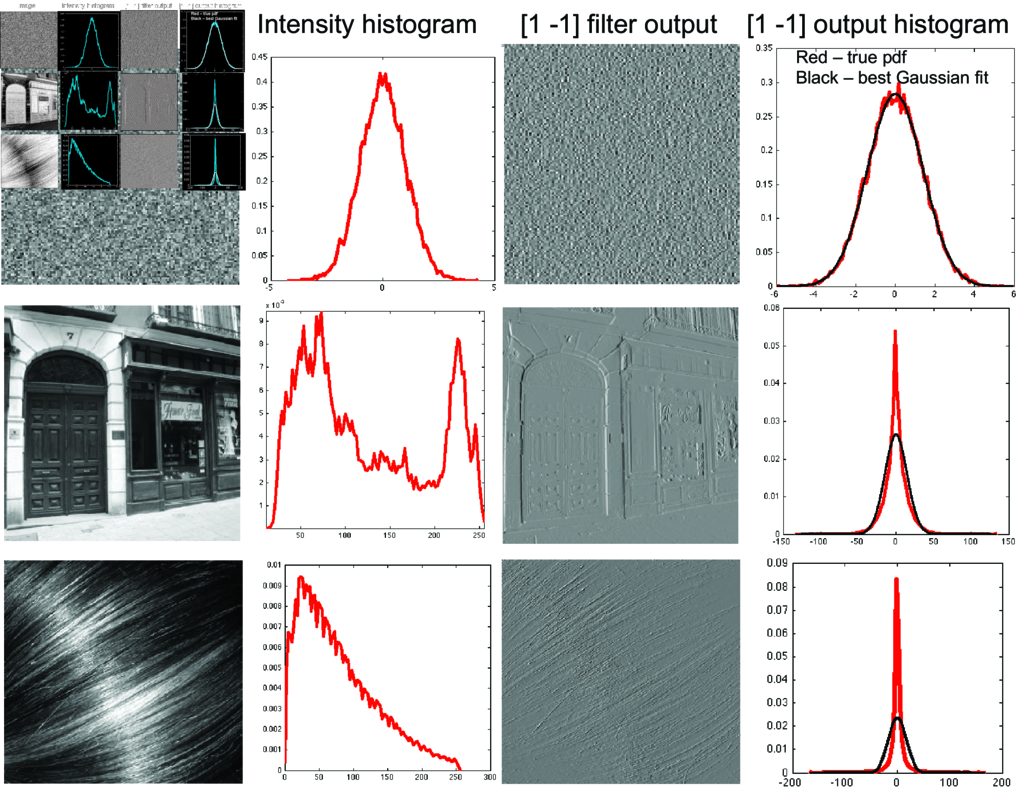
\includegraphics[width=1\linewidth]{figures/statistical_image_models/examplesderivativedistributions.eps}
} 
\caption{Comparison of histograms of images from different visual worlds (replace hair with clouds). Add image of leaves on the ground.} 
\label{fig:derivativesdistributions}
\end{figure}



\subsubsection{A remarkable property of image derivatives}
~\\

What what make the non-gaussianity of image derivatives really important is that the output distribution could be parametrized by a simple function:
\begin{equation}
p(x) = \frac{\exp \left(- \left| x/s  \right|^r \right)}{2s/r \Gamma(1/r)}
\label{eq:derdist}
\end{equation}

This function is called the Generalized exponential distribution. It has two parameters: the exponent $r$ which changes the shape of the distribution and $s$ which affects the variance. This distribution fits remarkably well the outputs of bandpass filters of natural images. 

Fig.~\ref{fig:generalizedgaussian} shows the shape of the distribution when changing the parameter $r$. $r=2$ gives the gaussian distribution. $r=1$ is called the laplacian distribution. When $r \to \infty$ the distribution converges to a uniform distribution in the range $\left[-s, s\right]$. And when $r \to 0$, the distribution converges to a delta function.
\begin{figure}[htpb]
\centerline{
\includegraphics[width=1\linewidth]{figures/statistical_image_models/generalizedgaussian.eps}
} 
\caption{Changing the exponent $r$ changes the shape of the distribution generating some special cases (gaussian, uniform, laplacian).} 
\label{fig:generalizedgaussian}
\end{figure}


Some properties of this distribution:
\begin{eqnarray}
mean = 0\\
var = \\
kurtosis = \\
\end{eqnarray}

Sometimes, vertical derivatives could be skewed due to illumination effects. Find one example.

%FIGURE: Compare the distribution obtained with different visual worlds (clouds, images, gaussian noise). Change the fit so that it uses the generalized gaussian.

In natural images, typical values of $r$ and in the range $\left[0.4, 0.8\right]$. 



There are other prior distributions that also fit well the data.



\subsubsection{The wavelet marginal model}
~\\

Now that we have seen that image derivatives have a special distribution for natural images, let's define a prior model that captures the distribution of image derivatives. Maximum entropy principle when only the marginals are specified:

\begin{equation}
p(\img) = \prod_{k} \prod_{x,y} p(h_k(\img, x,y))
\label{eq:waveletmodel}
\end{equation}
This model assumes that all the output values of all the filters are independent.

Observations: if $r = 2$, then this model becomes the gaussian model.


%\subsubsection{Examples}
%
%
%Example of a 1D step edge and sharpening. See the effect of p in what is the best solution.
%

First, what is the most likely image under the model eq.~\ref{eq:waveletmodel}. It is a constant image. 

%\begin{examples} {\bf step edge}

To build an intuition on what types of image structures are more likely under the wavelet marginal model, let's consider a simple 1D image:
\begin{equation}
\img = \left[1,~ 1,~ 1,~ a,~ 0,~ 0,~ 0\right]
\end{equation}
Different values of $a$ will produce different types of steps. For instance, setting $a=1$ or $a=0$ will produce a sharp step edge. Setting $a=0.5$ will produce a smooth step signal. What is the value of $a$ that maximizes the probability of this 1D image under the wavelet marginal model? 

First we need to specify the prior distribution. For this example we will use a model specified by a single filter with the form $[-1, 1]$, and we will use the distribution given by eq.~\ref{eq:derdist}. In this case, we can write the wavelet marginal model in close form. Applying the filter $\left[-1, 1\right]$ to the 1D signal and using mirror boundary conditions, results in:
\begin{equation}
h(\img) = \left[0,~0,~ 0,~ 1-a,~ a,~ 0,~ 0\right]
\end{equation}

Now, we can use Eq.~\ref{eq:waveletmodel} and obtain the probability of $\img$ as a function of $a$:
\begin{eqnarray}
p(\img) = \prod_{x} p(h(\img, x)) = \\
\frac {\exp \left(- \left| (1-a)/s  \right|^r \right) \exp \left(- \left| a/s  \right|^r \right)}{(2s/r \Gamma(1/r))^7} = \\
\frac{1}{(2s/r \Gamma(1/r))^7} \exp - \frac{\left| 1-a \right|^r+\left| a \right|^r} {s^r}  
\end{eqnarray}
the first factor only depends on $r$. The second factor depends on $a$ and $r$. We are interested in seeing the values of $a$ that maximize $p(\img)$ for each value of $r$. Therefore, only the second factor is important for this analysis. The next figure plots the value of the second factor as we vary $a$ and $r$. The red line represent the places where the function reaches a maximum as a function of $a$ for each value of $r$.

\begin{figure}[htpb]
\centerline{
\includegraphics[width=.6\linewidth]{figures/statistical_image_models/best_a_s1.eps}
} 
\caption{Best values of $a$ that maximize the probability of the 1D image $\left[1,~ 1,~ 1,~ a,~ 0,~ 0,~ 0\right]$ under the wavelet prior model.} 
\label{fig:best_a}
\end{figure}

For $r=2$ the best value of $a$ is $a=0.5$, and this solution is the best for any value of $r>1$. For $r=1$, any value $a \in \left[0,1\right]$ is equally good, and $p(\img)$ decreases for values of $a$ outside that range. And for $r<1$, the best solution is for $a=0$ or $a=1$. Therefore, values of $r<1$ prefer sharp step edges. Note that $a=0$ and $a=1$ are both the same step edge translated by one pixel. 

%\end{examples} 
%
%\begin{examples}
%What happens if the signal has the form: $\img = \left[0,~ 1,~ 2,~ a,~ 4,~ 5,~ 6\right]$
%\end{examples} 
%
%\begin{examples}
%What happens if the signal has the form: $\img = \left[0,~ 0,~ 0,~ a,~ 0,~ 0,~ 0\right]$. (solution: $a=0$ for all $r$).
%\end{examples} 
%
%\begin{examples}
%What happens if we define other filters than $\left[-1, 1\right]$. For instance $\left[-1,~ 2,~ -1\right]$.
%\end{examples} 
%
%\example{Superresolution}
%
%\begin{equation}
%{\bf a} = [a_0,~a_1,~ a_2,~ a_3,~ a_4,~ a_5,~ a_6,~a_7]
%\end{equation}
%
%but we observe the signal:
%\begin{equation}
%{\bf b} = [b_0,~ b_1,~ b_2,~ b_3]
%\end{equation}
%obtained by filtering $\bf a$ with a filter $[1,~1]$ and then downsampling by a factor of 2. The process of going from $\bf a$ to $\bf b$ is linear.
%\begin{eqnarray*}
%b_0 = a_0+a_1\\
%b_1 = a_2+a_3\\
%b_2 = a_4+a_5\\
%b_3 = a_6+a_7\\
%\end{eqnarray*}
%
%Our goal is to recover the signal $\bf a$.
%
%\begin{equation}
%\bf a ^* = argmax_{\bf a} P(\bf a ~|~ \bf b)  = \frac{P(\bf b ~|~ \bf a) P(\bf a)}{P(\bf b)}
%\end{equation}
%
%If we consider only the feasible solutions, then the only term that matters to select the solution is the prior $P(\bf a)$.
%
%\begin{equation}
%h({\bf a}) = [0,~a_1-a_0,~ a_2-a_1,~ a_3-a_2,~ a_4-a_3,~ a_5-a_4,~ a_6-a_5,~ a_7-a_6]
%\end{equation}
%
%\begin{equation}
%h({\bf a}) = [0,   ~b_0-2 a_0, ~
%                    a_2-a_1,~ b_1-2 a_2,~ 
%                    a_4-a_3,~ b_2- 2 a_4,~ 
%                    a_6-a_5,~ b_3- 2 a_6]
%\end{equation}
%
%\begin{eqnarray}
%\log p({\bf a}) = \sum_{x} \log p(h(\bf a, x)) = \\
%- \left | (b_0-2 a_0)/s  \right|^r
%- \left | (a_2-a_1)/s  \right|^r - \left | (b_1-2 a_2)/s  \right|^r
%- \left | (a_4-a_3)/s  \right|^r - \left | (b_2-2 a_4)/s  \right|^r
%- \left | (a_6-a_5)/s  \right|^r - \left | (b_3-2 a_6)/s  \right|^r
%\end{eqnarray}

%\begin{examples}{\bf Image impainting}
%
%2D image with a missing block in the center.
%
%It is like having boundary conditions.
%
%$I = I_b \cup I_c$
%
%$p(I_c ~|~ I_b)$
%\end{examples}
%
%\begin{examples}{\bf Most natural image}
%Find the image from a database that maximizes the prior... What is the most natural image? Figure: show sorted images according to the prior.
%\end{examples}
%
%
%\begin{examples}{\bf Superresolution}
%One example for which we can not derive things analytically. Use iterative weighted least square to do inference. Check effect on the exponent p on the solution.
%\end{examples}
%
%


\section{Sparsity}

Talk about Field and Olshausen, and establish parallelism with CNN.


\subsubsection{Cooring: Denoising with the wavelet model}
~\\

Deduce Wavelet thresholding using the bayesian model.

In the case of $\left[-1, 1\right]$ derivatives we can transform the image, then apply the prior to the derivatives, and then reverse the transformation. 

%
%\subsubsection{Retinex}
%
%Try a sequence of models:
%
%1) gaussian
%
%2) laplacian
%
%3) laplacian + gaussian on second order derivatives
%
%
%
%is one step beyond denoting...
%
%Craik-O'Brien-Cornsweet effect
%
%
%\begin{figure}[htpb]
%\centerline{
%\includegraphics[width=1\linewidth]{figures/statistical_image_models/Cornsweeteffect.eps}
%} 
%\caption{Cornsweet effect.} 
%\label{fig:Cornsweeteffect}
%\end{figure}
%




%\subsection{Gaussian scale mixtures}


%\section{Patch based models}
%
%How do non-parametric image models fit in this?







%\section{Generative models in vision}
%
%As a more challenging task: a really complete model. Can it be done? I think there is a CNN by Renato trying to build also priors for images. Describe it here.
%
%Explaining away, sufficient statistics, nuisance parameters, ...

%
%
%\section{Applications of statistical image models}
%
%
%\subsection{Camera motion removal}
%
%\subsection{Separating image into intrinsic images}
%
%\subsection{Color demosaicing}
%
%
\section{Concluding remarks}

The models presented here do not try to understand the content of the pictures, and  the rules about the structure of images is rather limited. However, this models are very powerful when used to solve challenging image processing tasks. %We will see here N examples


